\documentclass[a4paper,12pt]{article}
\usepackage[utf8]{vietnam}
\usepackage{geometry}
\usepackage{graphicx}
\usepackage{amsmath}
\usepackage{titlesec}
\usepackage{tikz}
\usepackage{enumitem}
\usepackage{fancyvrb}
\usepackage{tocloft}
\usepackage[hidelinks]{hyperref}
\usepackage{etoolbox}
\usepackage{float}

\geometry{a4paper, margin=1in}
\pagestyle{plain}

\begin{document}

\begin{tikzpicture}[remember picture, overlay]
    \draw[line width=3pt] ([shift={(1cm,1cm)}]current page.south west) rectangle ([shift={(-1cm,-1cm)}]current page.north east);
    \draw[line width=1pt] ([shift={(1.1cm,1.1cm)}]current page.south west) rectangle ([shift={(-1.1cm,-1.1cm)}]current page.north east);
\end{tikzpicture}

\begin{center}

    {\Large \textbf{POSTS AND TELECOMMUNICATIONS INSTITUTE OF TECHNOLOGY}} \\
    \vspace{0.2cm}
    {\small UNIT: INFORMATION TECHNOLOGY} \\
    \vspace{0.5cm}
    
    
\includegraphics[width=0.4\textwidth]{logo.png} \\
    \vspace{0.5cm}
    
    {\Large \textbf{ASSIGNMENT REPORT}} \\
    \vspace{0.2cm}
    {\large \textbf{SUBJECT: PYTHON}} \\
    \vspace{1.5cm}
    
    \begin{center}
    \begin{tabular}{ll}
    \textbf{LECTURER:} & Kim Ngoc Bach \\
    \textbf{CLASS:} &  B23CQCE04-B\\
    \textbf{STUDENT:} & Pham Quang Vinh - B23DCCE100
    \end{tabular}
    \end{center}
\end{center}
\newpage

\renewcommand{\figurename}{Image}

\renewcommand{\contentsname}{Contents}

\setlength{\cftbeforesecskip}{12pt}       
\setlength{\cftbeforesubsecskip}{8pt}     

\setlength{\cftbeforesecskip}{20pt}
\setlength{\cftbeforesubsecskip}{12pt}

{\large
\tableofcontents
}
\newpage

\section*{I. Requirements}
\phantomsection
\addcontentsline{toc}{section}{I. Requirements}
\begin{itemize}[label= {-}, leftmargin= 1cm]
    \subsection*{Problem 1}
    \phantomsection
    \addcontentsline{toc}{subsection}{Problem 1}
        \begin{itemize}[label= {-},  leftmargin= 2cm]
            \item Collect data of player who have played more than 90 minutes in the 2024 - 2025 English Premier League season.
        \end{itemize}

    \subsection*{Problem 2}
    \phantomsection
    \addcontentsline{toc}{subsection}{Problem 2}
        \begin{itemize}[label= {-}, leftmargin= 2cm]
            \item Identify the top 3 best and worst players for each statistic.
            \item  Find the median, mean, and standard deviation for each team.
            \item  Plot histogram for 3 offense and defense statistics.
        \end{itemize}

    \subsection*{Problem 3}
    \phantomsection
    \addcontentsline{toc}{subsection}{Problem 3}
        \begin{itemize}[label= {-}, leftmargin= 2cm]
            \item Use the K-means algorithm to classify the player.
            \item Use PCA to reduce the data dimensions to 2 and plot a 2D cluster.
        \end{itemize}

    \subsection*{Problem 4}
    \phantomsection
    \addcontentsline{toc}{subsection}{Problem 4}
        \begin{itemize}[label= {-}, leftmargin= 2cm]
            \item Collect player transfer values who have played more than 900 minutes in the 2024 - 2025 EPL season.
            \item Propose a method for estimating player values and how to select features and models.
        \end{itemize}

\end{itemize}
From above requirements, I can see that we need to collect player's data and analyze the data then find the best player, worst player, best team or worst team. Beside, we also need to classify the player and visualize it by using PCA method, propose a method to estimate player values. To do that we'll need the data source and methods:

\begin{itemize}[leftmargin= 1cm]
    \item Data source:
        \begin{itemize}[label={}, leftmargin= 1cm]
            \item Player data: \url{https://fbref.com/en/}
            \item Player transfer values: \url{https://example.com}
        \end{itemize}
    \item Libraries, tools:
        \begin{itemize}[label= {}, leftmargin= 1cm]
            \item For scraping data: Selenium, BeautifulSoup, Requests
            \item For analyze and process data: Pandas, Numpy, Unidecode
            \item For clustering and estimating: Scikit-learn
            \item For ploting: Matplotlib, Seaborn
        \end{itemize}
\end{itemize}

\newpage
\section*{II. Solutions}
\phantomsection
\addcontentsline{toc}{section}{II. Solutions}
\begin{itemize}[label= {*}, leftmargin= 1cm]
    \subsection*{1) Problem 1}
    \phantomsection
    \addcontentsline{toc}{subsection}{1) Problem 1}
    \item {\Large Idea:}
    \begin{itemize}[label= {-}, leftmargin= 1cm]
        \item Use selenium and webdriver to crawl data from web
        \item Filter and get necessary data
    \end{itemize}
    \item {\Large Details:}
    \begin{itemize}[label= {}, leftmargin= 1cm]
        \item a) Selenium configuration:

        \begin{figure}[h]
            \centering
            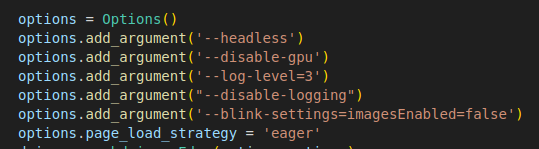
\includegraphics[width=0.7\linewidth]{options.png}
        \end{figure}
        I configured the Edge browser with these following options to optimize runtime of the code:
        \begin{itemize}[label= {-}]
            \item \textbf{Headless mode:} run web browser without displaying the interface.
            \item \textbf{Disable GPU and images:} Speeds up page loading
            \item \textbf{Page load strategy:} Waits only for the DOM to load (doesn't wait for all resources)
        \end{itemize}
        
        \item b) Collect basic player data:

        \begin{Verbatim}[fontsize=\footnotesize, xleftmargin=-1cm]
        rows = WebDriverWait(driver, 20).until(
            ec.presence_of_all_elements_located((By.CSS_SELECTOR, 'table#stats_standard 
            tbody > tr:not(.thead):not(.rowSum)'))
        )   
        \end{Verbatim}
        I used it instead of:
        
        \begin{Verbatim}[fontsize=\footnotesize, xleftmargin=-1cm]
        rows = driver.find_elements(By.CSS_SELECTOR, 'table#stats_standard 
        tbody > tr:not(.thead):not(.rowSum)')
        \end{Verbatim}
        
        to advoid errors which the necessary data haven't been loaded yet.
        The lines of code above will collect all of rows contain player in the league excepted non-player elements. Next, I defined the data structures by using a dictionary \textbf{player\_statistic} maps columns names to their corresponding \textbf{data-stat} attreibutes in the HTML table. For instance:

        \begin{Verbatim}[fontsize=\footnotesize, xleftmargin=-1cm]
            'Player': "player",
            'Nation': "nationality",
            'Team': "team",
            'Pos': "position",
            'Age': "age",
        \end{Verbatim}      

        Then for each row, the script extracts data for all columns defined in \textbf{player\_statistic} and player with playing time less than 90 minutes will be excluded. But at first I need to changed 'Min' columns from \textbf{'object'} to \textbf{'float'} that I can compare with 90. The extracted data is sorted in a \textbf{Pandas DataFrame} to process easier later. Additional adding a \textbf{First\_name} columns by splitting the player's fullname and sorting the DataFrame by \textbf{First\_name} columns but in case it's the same I sorted further by \textbf{Player (Name)}.\\
        
        In additional to the "Standard Stats" table, data is collected from serveral other tables on the \textbf{fbref.com} website. These tables provide specialized statistics, such as goalkeeping performance, shooting accuracy, passing metrics, and more. I also create a dictionary has the same structure to \textbf{player\_statistic} to get the information and compile into one list named \textbf{target} which include:
        \begin{itemize}[label= {+}, leftmargin= 1cm]
            \item id of the stactic table in HTML of the website
            \item \textit{data-stat} for each statistic that I need
            \item a link lead to the website contain the statistic table
        \end{itemize}
        Example:
        \begin{Verbatim}[fontsize=\footnotesize, xleftmargin=-1cm]
            ('table#stats_keeper',  gk_statistic, 'https://fbref.com/en/comps/9/keep
            ers/Premier-League-Stats')
        \end{Verbatim}
        \vspace{0.5cm}

        To get data from every table I built a function named \textbf{get\_statistic} with arguments are the data-stat dictionary and all rows of player and return a DataFrame. After collecting data from all tables, the script consolidates the data into a single DataFrame(\textbf{df\_all}) with using the \textbf{reduce} function is used to merge all DataFrame on \textbf{Player} and \textbf{Team} columns because I realized that if I merge on \textbf{Player} only there were still some duplicate name. Why did this happend? Because some players tranfered to other team during the season so it would be duplicated. Beside there still had missing values and it is replaced by \textbf{'N/a'} values.
        \vspace{0.5cm}

        The reslult file is a CSV file(\textit{resluts.csv}) containing details statistics of all player in 2024 - 2025 English Premier League season. It is well-organized and ready for further analysis, such as performance evaluation, trend analysis, or predictive modeling.
        
    \end{itemize}
    \item {\Large Conclusion:}
    \begin{itemize}[label= {}, leftmargin= 1cm]
        \item The script successfully collects and processes detailed player statistics from the fbref.com website. The resulting CSV file provides valuable insights into player performance and can be used for various analytical purposes.
    \end{itemize}
    \newpage

    \subsection*{2) Problem 2}
    \phantomsection
    \addcontentsline{toc}{subsection}{2) Problem 2}
    \item {\Large Idea:}
    \begin{itemize}[label= {-}, leftmargin= 1cm]
        \item Reuse the data is collected in the Problem 1 
        \item Use pandas to identify best player, team, find median, mean, ...
        \item Group the data by Team and plot it
    \end{itemize}
    \item {\Large Details:}
    \begin{itemize}[label= {}, leftmargin= 1cm]
        \item a) Identify top 3 best and worst player for each statistic
        \vspace{0.5cm}
        
        First of all I reused the data that I collected in the Prolblem 1 to process and handling missing data with any antries with 'N/a' are treated as NAN and they are \textbf{replaced with 0} using \textbf{filla(0)}. I got statistics is all columns starting from the 10th column (\textbf{df.columns[9:]}) are treated as \textbf{statistical metrics} because I want to remove some unnecessary statistics like \textbf{Name, Age, Nationality, etc} a and then \textbf{converted to numeric} to ensure proper sorting and comparison.
        \vspace{0.5cm}
        To identify top 3 , I looped through each statistics and sort the DataFrame in descending order by the statistic. Select Top 3 (\textbf{top3}) for the highest values and Bottom 3 (\textbf{bottom3}) for the lowest values with \textbf{head} and \textbf{tail} function in Pandas. A new column is also added to recognize between best and worst player for each statistics. 

        \begin{Verbatim}[fontsize=\footnotesize, xleftmargin=-1cm]
            top3 = sorted_df.head(3).copy()
            bottom3 = sorted_df.tail(3).copy()
        \end{Verbatim}

        The results file is a table that is concatenated by the top and bottom 3 players for each statistic, is appended (\textbf{'a'} mode) to a text file and clear heading are added for each statistic.
        \vspace{0.8cm}
        

        \item b) Find median, mean and standard deviation for each team 
        \vspace{0.5cm}
        
        \verb|df = df.apply(pd.to_numeric, errors='ignore')|
        
        I tried to \textbf{convert all columns to numeric} if possible (errors= 'ignore' keeps non-convertible columns unchanged). 

        \begin{Verbatim}[fontsize=\footnotesize, xleftmargin=-1cm]
            median_df = df.groupby('Team', as_index= False).median(numeric_only= True)
            mean_df = df.groupby('Team', as_index= False).mean(numeric_only= True)
            std_df = df.groupby('Team', as_index= False).std(numeric_only= True)
        \end{Verbatim}

        To calculate aggregation, I group the data by \textbf{'Team'} and only \textbf{numeric columns} are considered (numeric\_only= True):
        \begin{itemize}[label= +, leftmargin= 1cm]
            \item \textbf{Median}(median\_df): Computes median of each numeric column for each team.
            \item \textbf{Mean}(mean\_df): Computes mean similarly.
            \item \textbf{Standard Deviation}(std\_df): Computes standard deviation.
        \end{itemize}

        Before merging the summary statistics, the script first drops irrelevant columns (\textit{'Unnamed: 0'}, \textit{'MP'}, and \textit{'Starts'}) from all three DataFrames. These columns are likely identifiers or values that are not meaningful for statistical aggregation. This step ensures that only useful numeric data is included in the subsequent calculations.
        \vspace{0.3cm}

        To build the combined table, I \textbf{initializes an empty dictionary} (combined\_dict) and iterates through each statistical column. For every statistic, it adds the corresponding \textbf{median}, \textbf{mean}, and \textbf{standard deviation} under clearly labeled new column names, such as 'Median of Goals', 'Mean of Goals', and 'Std of Goals'. The 'Team' column is specially handled to remain unchanged as a consistent anchor for the data. After organizing the data, I concatenates all values horizontally (axis=1) into a new DataFrame (combined\_df) and writes the final result to results2.csv, keeping the index in the output file.
        \vspace{0.8cm}
        

        \item c) Plot histogram of 3 offense and defense statistics
        \vspace{0.5cm}

        I choose \textbf{Goals(\textit{Gls}), Expected Goals(\textbf{xG}), Shot-creation Action per 90(\textit{SCA90})} as offense statistics and \textbf{Tackle(\textit{Tkl}), Interceptions(\textbf{Int}),}\\
        \textbf{Blocks(\textit{Blocks})} as defense statistics by removing commas and ensuring all values are numeric. Invalid values are coerced to NaN using errors='coerce'. 
        
        A list of unique teams is created from the 'Team' column. Then, a dictionary (teams\_dict) is generated, where each team is associated with its corresponding subset of the DataFrame.

        For plotting and saving histograms, I created subplots in a 3x7 grid for each statistic. The first plot shows the overall Premier League distribution, while the remaining plots display each team's distribution. Each histogram is saved as a .png file in the Problem2/Data directory, with filenames corresponding to the statistic (e.g., Gls.png), making it easy to compare distributions across teams and the league.
        \vspace{0.3cm}
        
        Here is the example:
        \begin{figure}[h]
            \centering
            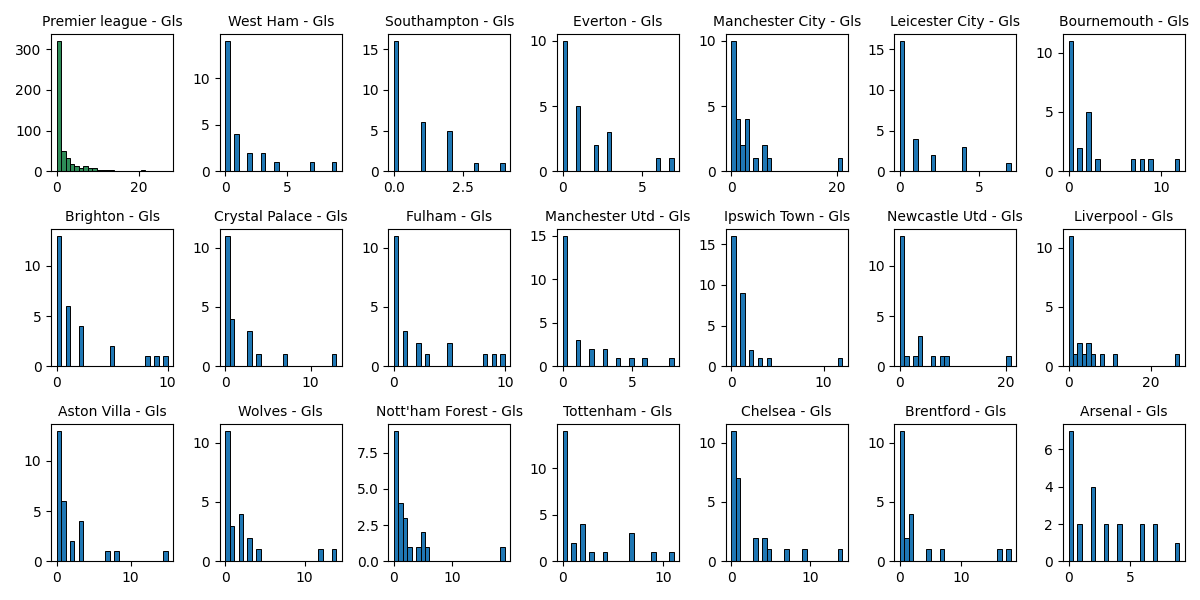
\includegraphics[width=0.7\linewidth]{Gls.png}
            \caption{Goals plotting}
        \end{figure}
        \newpage        
        
        \item d) Identify the team with the highest score
        \vspace{0.5cm}
        
        After calculated median, mean, and standard deviation from above part, we can easily find which team is leading in some statistics by calculate their mean in each statistic and find the team lead the most 
        \vspace{0.2cm}
        
        \textbf{Data Preprocessing}\\
        The script begins by loading data from a CSV file (\texttt{'Problem1/results.csv'}) and handling missing values, specifically replacing any \texttt{'N/a'} entries with 0. It then drops the \texttt{'Unnamed: 0'} column, which is likely an index or irrelevant identifier. The \texttt{'Age'} column is also cleaned by extracting only the lower bound of the age range (if provided in a range format like '25-29').
        \vspace{0.3cm}
        
        \textbf{Handling Statistical Columns}\\
        Next, the script identifies numeric columns in the dataset and addresses potential formatting issues. It removes commas from numbers (commonly used for thousands separators) and ensures that non-numeric values are properly coerced to NaN where necessary. This ensures that all numeric columns are clean and ready for analysis.
        \vspace{0.3cm}
        
        \textbf{Splitting Data by Teams}\\
        The data is then grouped by team using a dictionary (\texttt{teams\_dict}), where each team’s data subset is stored as a separate DataFrame. This allows the script to perform calculations for each team individually, making it easier to compare team performances across various statistics.
        \vspace{0.3cm}
        
        \textbf{Calculating Highest Scores}\\
        For each statistical column, I calculates either the sum or the mean, depending on the type of statistic:
        \begin{itemize}
            \item For statistics like yellow cards (\texttt{CrdY}) and red cards (\texttt{CrdR}), the script calculates the sum to determine which team has the lowest score (fewer cards).
            \item For other statistics (e.g., goals, assists), the script calculates the mean to identify which team has the highest average score.
        \end{itemize}
        For each statistic, the team with the highest value (or lowest for card statistics) is identified, and the result is printed for clarity.
        \vspace{0.3cm}

        \newpage
        \textbf{Determining the Best Team}\\
        Finally, I uses the \texttt{Counter} class to count how many times each team had the highest score across all statistics. The team with the most highest scores is considered the best performing team of the 2024-2025 Premier League season. The script then prints the name of this team along with the number of statistics in which they had the highest score.

        \begin{figure}
            \centering
            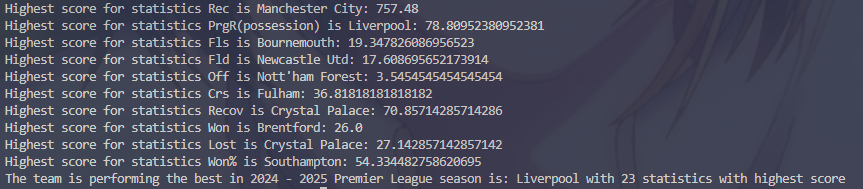
\includegraphics[width=0.7\linewidth]{highest_score.png}
            \caption{Team with hight score}
        \end{figure}
        
    \end{itemize}
    \item {\Large Conclusion:}
    \begin{itemize}[label= {-}, leftmargin= 1cm]
        \item identify\_top3 is a solid foundation for \textbf{automated performance reporting} across many statistics. With minor refinements, it could become a reusable tool for deeper player performance analysis across various datasets.
        \item find\_median\_mean\_std effectively summarizes team performance with central tendency and dispersion measures. It is robust and clear, but with a few refinements, it can be made more efficient, flexible, and professional for repeated use.
        \item The determine the best team provides insights into which team cons istently performs the best in various metrics across the season, offering a clear picture of top performers in the Premier League.
    \end{itemize}
    \newpage

    \subsection*{3) Problem 3}
    \phantomsection
    \addcontentsline{toc}{subsection}{3) Problem 3}
    \item {\Large Idea:}
    \begin{itemize}[label= {-}, leftmargin= 1cm]
        \item Use elbow and silhouette method to find k clustes.
        \item Use KMeans clustering from scikit-learn to group player base on their statistics.
        \item Use PCA from scikit-learn to reduce data dimension to 2.
    \end{itemize}
    \item {\Large Details:}
    \begin{itemize}[label= {}, leftmargin= 1cm]
        \item a) Find number of clusters
        First, the dataset used in this analysis was loaded from a CSV file named that I collected in Problem 1, which contains various performance metrics for football players. To ensure the dataset was suitable for clustering, a thorough preprocessing pipeline was applied. Initially, several non-numerical or identifying columns were removed from the dataset, specifically \textbf{Unnamed: 0, Player, Nation, Team, Pos, Age, and Min}, as these either represented categorical identifiers or provided information not directly useful for unsupervised clustering.

        Following this, the remaining data was examined for formatting inconsistencies. It was noted that several numerical values were stored as strings containing commas, such as "1,234". To resolve this, each object-type column was converted to a float after removing comma characters. This step ensured all values were properly treated as numerical data types. Next, the dataset was checked for missing values. Any missing entries were imputed with the mean of the respective column using
        
        \vspace{0.1cm}
        \verb|df.fillna(df.mean(numeric\_only=True))|
        \vspace{0.1cm}
        
        a method that preserves the central tendency of the data while allowing the clustering algorithm to function without disruption. At the end of this preprocessing phase, the dataset consisted exclusively of clean, numerical data ready for unsupervised learning.

        To identify the optimal number of clusters kk for the KMeans algorithm, two commonly used evaluation techniques were implemented: the \textbf{Elbow Method} and the \textbf{Silhouette Score Method}.
        \vspace{0.3cm}
        
        \textbf{Elbow Method}
        \begin{Verbatim}[xleftmargin=-1cm]
            wscc = []
            k_values = range(1, 11)
            
            for k in k_values:
                kmeans = KMeans(n_clusters= k, random_state= 42)
                kmeans.fit(df)
                wscc.append(kmeans.inertia_)
        \end{Verbatim}  
        \vspace{0.3cm}
        
        I created a list named \textbf{wscc}(Within-Cluster Sum of Squares), which measures the total distance between each point and the centroid of its assigned cluster, it is calculated by \textbf{kmeans.inertia\_} attribute of scikit-learn. The WCSS is expected to decrease as k increases since more clusters result in tighter groupings. This method involves fitting the KMeans algorithm on the dataset for a range of cluster count from \textbf{\textit{k} = 1} to \textbf{\textit{k} = 10}. However, there comes a point where the marginal gain in reducing WCSS diminishes. This point, referred to as the "elbow," is typically considered a good estimate for the optimal number of clusters.
        \vspace{0.3cm}

        I visualized this method to a plot to provides a clear way to identify the elbow point by looking for a change in the slope of the curve - where the curve begin to flatten significantly.
        
        \begin{figure}[h]
            \centering
            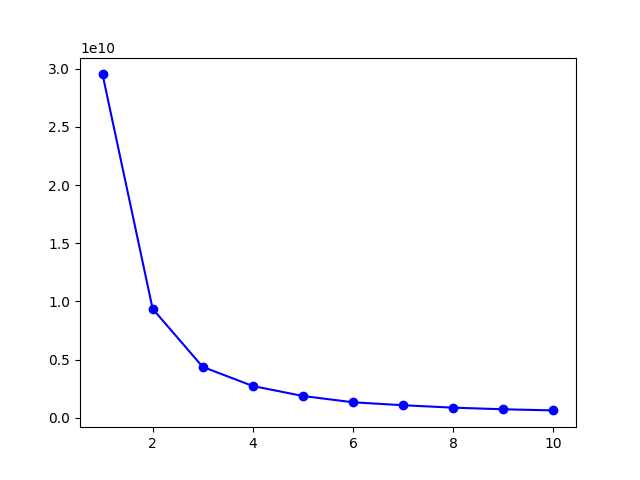
\includegraphics[width=0.7\linewidth]{elbow_method.png}
            \caption{Elbow method}
        \end{figure}
        
        \vspace{0.5cm}

        \textbf{Silhouette Score Method}
        \begin{Verbatim}[xleftmargin=-1cm]
            silhouette = []

            for k in range(2, 11):
                kmeans = KMeans(n_clusters= k, random_state= 42)
                label = kmeans.fit_predict(df)
                score = silhouette_score(df, label)
                silhouette.append(score)
        \end{Verbatim}  
        \vspace{0.3cm}
        
        To find the most accurate number of clusters in KMeans, I also used Silhouette method. The Silhouette Score is a more advanced metric that evaluates the quality of clustering by measuring how similar an object is to its own cluster compared to other clusters. The score ranges from -1 to 1, with higher values indicating better-defined and more cohesive clusters. For this method, the KMeans algorithm was fitted for cluster counts ranging from \textbf{\textit{k} = 2} to \textbf{\textit{k} = 10}, and for each value of \textbf{\textit{k}}, the average silhouette score was calculated across all samples and the score will be saved to a list(\textbf{silhouette}).
        \vspace{0.3cm}
        
        I also visualized it and peaks in the silhouette score curve are particularly informative, as they point to the number of clusters that best balance intra-cluster tightness and inter-cluster separation. Unlike the Elbow Method, the Silhouette Score offers a quantitative measure of clustering performance and can provide stronger justification for selecting a particular \textbf{\textit{k}}.

        \begin{figure}[h]
            \centering
            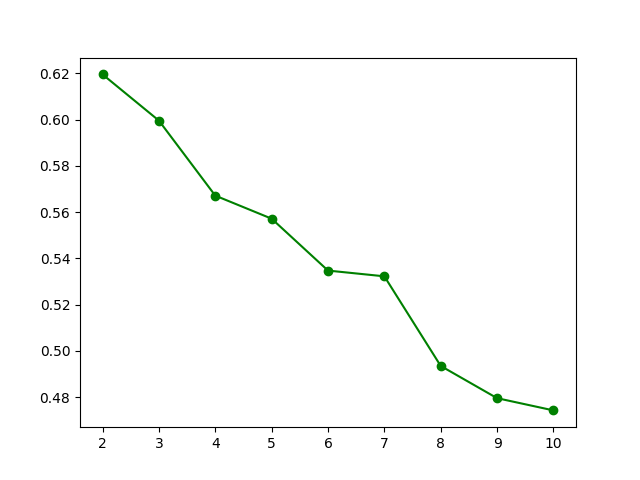
\includegraphics[width=0.7\linewidth]{silhouette_method.png}
            \caption{Silhouette score method}
        \end{figure}
        
        \vspace{0.5cm}

        Upon evaluating the WCSS curve generated by the Elbow Method, it appears that the rate of decrease in WCSS begins to level off significantly around \textbf{\textit{k} = 3} or \textbf{\textit{k} = 4} suggesting that this range captures the underlying structure of the data well without unnecessary complexity. While the WCSS continues to decline beyond these values, the marginal improvement is minimal, indicating diminishing returns for higher cluster counts.
        \vspace{0.3cm}

        In parallel, the Silhouette Score analysis further reinforces this observation. The silhouette score typically peaks \textbf{\textit{k} = 2} to \textbf{\textit{k} = 3} at with values dropping off for both smaller and larger cluster counts. This suggests that clustering the dataset into three or four groups yields the most coherent and well-separated clusters. These findings align with the visual and statistical indications from both methods, lending confidence to the selection of this cluster range.
        \vspace{0.3cm}

        Through 2 methods above I found that \textbf{\textit{k} = 3} is the most accurate number of clusters to group player base on their statistics. With \textbf{\textit{k} = 3}, I think they will be grouped 3 type of player:
        \begin{itemize}[label= {+}, leftmargin= 1cm]
            \item First is players with high offense stats like goals, expected goals, shot on target, ...
            \item Second is players with high assist stats like assist, completed pass, key pass, ...
            \item Third is players with higt defense stats like tackle, block, ...
        \end{itemize}

        \item b) Reduce the data dimensions to 2
        \vspace{0.3cm}

        After identifying the optimal number of clusters, the next step involved visualizing the clustering results in a lower-dimensional space. Since the original dataset contains a relatively high number of numerical features, directly visualizing the clusters in raw feature space is not practical. Therefore, \textbf{Principal Component Analysis (PCA)} was employed to reduce the dimensionality of the dataset while retaining as much variance as possible.
        \vspace{0.3cm}

        \begin{Verbatim}[xleftmargin= -1cm]
            missing_rate = df.isna().mean()
            df = df.loc[:, missing_rate < 0.3]
            
            df.fillna(df.mean(numeric_only= True), inplace= True)
        \end{Verbatim}  
        \vspace{0.3cm}
        Before applying PCA, the dataset underwent further refinement. Columns with more than 30\% missing values were removed to maintain data integrity. the remaining missing values were filled using the column-wise mean, a common imputation method that preserves the overall distribution. 
        \vspace{0.3cm}

        \begin{Verbatim}[xleftmargin= -1cm]
            scaler = StandardScaler()
            df_scaled = scaler.fit_transform(df)
        \end{Verbatim}
        The features were then scaled using \textbf{StandardScaler} to standardize them with zero mean and unit variance. Standardization is essential before PCA because it ensures that all features contribute equally to the principal components, especially when they are measured on different scales.
        \vspace{0.3cm}

        \begin{Verbatim}[xleftmargin= -1cm]
            pca = PCA(n_components= 2)
            df_pca = pca.fit_transform(df_scaled)
        \end{Verbatim}
        \vspace{0.3cm}

        The PCA algorithm was applied with \textbf{n\_components=2} to project the data into a two-dimensional space. This 2D representation captures the major variance in the data and provides a meaningful structure for visualization. Following dimensionality reduction, the KMeans clustering algorithm was re-applied on the PCA-transformed data using three clusters, as previously determined by the Elbow and Silhouette methods.
        \vspace{0.3cm}

        To interpret and present the clustering results, a scatter plot was generated, in which each point represents a player in the two-dimensional PCA space. The color of each point corresponds to its assigned cluster, providing a visual summary of the separation and cohesion between groups. 
        \newpage
        
        \begin{figure}[h]
            \centering
            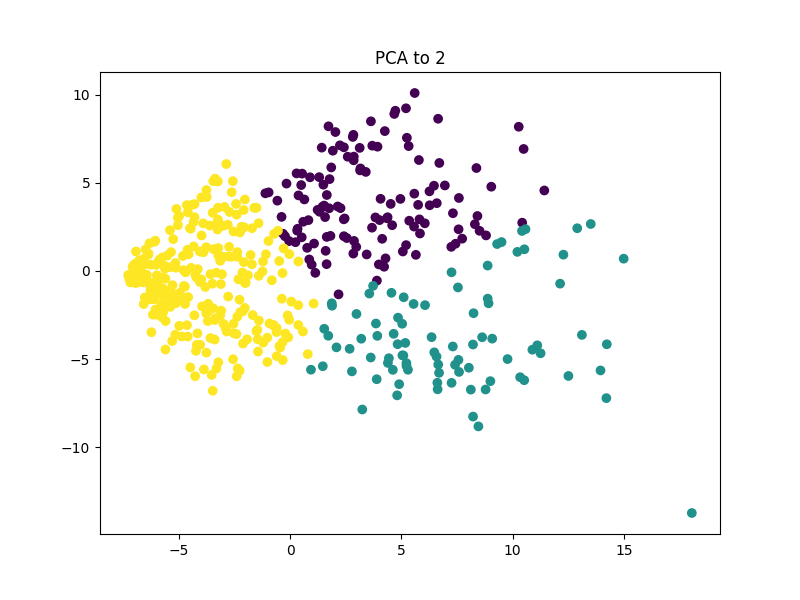
\includegraphics[width=0.7\linewidth]{PCA.png}
            \caption{Use PCA to reduce the data dimension to 2}
        \end{figure}
        
        \vspace{0.3cm}
        
    \end{itemize}
    \item {\Large Conclusion:}
    \begin{itemize}[label= {-}, leftmargin= 1cm]
        \item Based on the Elbow and Silhouette methods, using \textbf{three or four clusters }is recommended. Three clusters offer broader groupings (e.g., defensive, midfield, attacking), while four clusters provide more detailed subgroups within those roles, balancing simplicity and insight.
        \item PCA was used to reduce the dataset to two dimensions, allowing for a clear visual representation of the KMeans clustering results. The resulting scatter plot showed distinct separation between clusters, confirming that PCA effectively preserved the structure of the data and made the clustering outcome easier to interpret.
    \end{itemize}
    \newpage

    \subsection*{4) Problem 4}
    \phantomsection
    \addcontentsline{toc}{subsection}{4) Problem 4}
    \item {\Large Idea:}
    \begin{itemize}[label= {-}, leftmargin= 1cm]
        \item Use selenium and webdriver to crawl data from web
        \item Use some supervised learning method to estimates player value like linear regression, logistic regression, ...
    \end{itemize}
    \item {\Large Details:}
    \begin{itemize}[label= {}, leftmargin= 1cm]
        \item a) Collect player transfer values for 2024 - 2025 season
        First, I had base url is https://www.footballtransfers.com/us/values/players/most-valuable-\\
        soccer-players/playing-in-uk-premier-league, it's also the first page which contain player transfer values. Every page from 2 to the end will add the number of the page into the end of the base link so I could loop through all the links easily. 
        \vspace{0.3cm}

        \begin{Verbatim}[fontsize=\footnotesize, xleftmargin= -2cm]
            rows = WebDriverWait(driver, 20).until(
                ec.presence_of_all_elements_located((By.CSS_SELECTOR, 'tbody#player-
                table-body > tr'))
            )

            players = []
            for i in range(len(rows)):
                try:
                    row = driver.find_elements(By.CSS_SELECTOR, 'tbody#player-table-body > tr')[i]
                    name = row.find_element(By.CSS_SELECTOR, 'td.td-player a').text.strip()
                    value = row.find_element(By.CSS_SELECTOR, 'span.player-tag').text.strip()
                    players.append({'Player': name, 'Values': value})
                except:
                    players.append({'Player': None, 'Values': None})
                    
            player_df = pd.DataFrame(players)
            df = pd.concat([df, player_df], ignore_index= True)
        \end{Verbatim}
        \vspace{0.3cm}
        
        For each page, the script locates the player table rows using CSS selectors and extracts both the player's name and their estimated transfer value. These values are stored in a list of dictionaries, which is then converted to a Pandas DataFrame. This process is repeated across all 22 pages and concatenated into a single dataset. I tried to get the \textbf{row} in \textbf{rows} I found but the DOM changed due to I couldn't get their name and transfer value. Therefore, I used 
        \vspace{0.3cm}

        \begin{Verbatim}[fontsize=\footnotesize, xleftmargin= -2cm]
            row = driver.find_elements(By.CSS_SELECTOR, 'tbody#player-table-body > tr')[i]
            name = row.find_element(By.CSS_SELECTOR, 'td.td-player a').text.strip()
            value = row.find_element(By.CSS_SELECTOR, 'span.player-tag').text.strip()
            players.append({'Player': name, 'Values': value})
        \end{Verbatim}
        \vspace{0.3cm}
        
        to take player data with try - except to avoid the case if I couldn't get the data, the programme would add nothing into the DataFrame instead of crashing.
        \vspace{0.3cm}

        To determine player whose playing time is greater than 900 minutes, I used the data in Problem 1 but it is collected in another website, so the structure is also different. That's mean, there're some player will be unmatch from 2 DataFrame. To ensure consistency and enable successful merging with the performance data, the player names are cleaned using a helper function named clean\_name. This function standardizes the names by:
        \begin{itemize}[label= {+}, leftmargin= 1cm]
            \item Converting to lowercase
            \item Removing accents using \textbf{unidecode}
            \item Replacing hyphens with spaces
            \item Stripping punctuation and retaining only the first and last name components (sorted alphabetically)
        \end{itemize}
        \vspace{0.3cm}

        Both datasets are augmented with a normalized Name column, enabling a fuzzy join via exact matching on cleaned names. A left join is performed to ensure only players present in both datasets (i.e., valuable and active players) are retained. After the merge, rows with missing values are dropped to ensure data integrity.

        Because of merging by clean\_name so it created unnecessary columns like \textbf{'Player\_x', 'Player\_y', ..} so unnecessary columns are removed, and the merged dataset is exported to a CSV file (transfer\_values.csv) for further analysis.
        \vspace{0.3cm}

        \item b) Estimating player values
        \vspace{0.3cm}

        To estimate player values effectively, I get the transfer values above and their statistics that I collected in the Problem 1. Start with narrow them dow using statisticaal and model-based techniques. The common feature groups include:
        \begin{itemize}[label= {+}, leftmargin= 1cm]
            \item \textbf{Performance stats:} goals, assist, xG, xA, shots, passes, tackles, interceptions, etc.
            \item \textbf{Playing time:} Minutes played, game started, age.
            \item \textbf{Position-specific metrics:} defender: clearances, aerial duels won; attackers: dribbles, key passes.
        \end{itemize}
        \vspace{0.3cm}
        
        About model selection, I approached the problem as a regression prooblem, where the target variable is the player's transfer values in milions of euros. There are some model that we can consider:
        \begin{itemize}[label= {+}, leftmargin= 1cm]
            \item \textbf{Linear Regression (Base line):} Easy to interpret, but limited with nonlinearities.
            \item \textbf{Ridge/Lasso Regression:} Adds regularzation, useful for reducing overfitting ans handling multicollinearity.
            \item \textbf{Random Forest Regressor:} Captures nonlinear relationships, robust to outliers.
            \item  \textbf{XGBoost or LightGBM:} More powerfull tree-based models, often best performance.
        \end{itemize}
        but for easy, I will choose Linear Regression.
        \vspace{0.3cm}

        First, we conducted data cleaning and preprocessing. All missing values were filled with zeros for simplicity, though in future iterations, more nuanced imputation methods could be explored. The \textbf{Values} column, originally in the format of '€X.M', was stripped of the euro symbol and the 'M' character to convert the values into pure floats. To handle positional data, we simplified the multi-position entries by extracting only the primary position (i.e., the first listed), and then applied one-hot encoding to convert categorical position data into numerical features.
        \vspace{0.3cm}

        \begin{Verbatim}[xleftmargin= -1.5cm]
            df = pd.get_dummies(df, columns=['Pos'])
            for col in df.columns:
                if df[col].dtype == 'object':
                    if df[col].str.contains(',').any():
                        df[col] = df[col].str.replace(',','').astype(float)
        \end{Verbatim}
        \vspace{0.3cm}

        We also ensured that all other relevant features were converted to numeric types, particularly those that might have contained comma-separated strings due to formatting inconsistencies. After preprocessing, we selected all numeric features—excluding the target variable—as our feature set for model training. And I add one-hot encoding columns is position to estimate exactly the values of a player because it has a strong influence. A striker with 10 goals is good. But a defender who scores 10 goals is crazy. Similarly, the tackling index of a defensive midfielder is more important than that of a striker. Without using Position, the model is prone to biased comparisons between positions. Position provides context for player activity, helping the model understand that: 5 goals by defender => higher value than 15 passes per game by striker => not so special.
        \vspace{0.3cm}

        The feature set was standardized using \textbf{StandardScaler} to ensure that all features contribute equally to the model, as unscaled features in linear regression can bias the coefficients toward features with larger numeric ranges.
        \begin{Verbatim}[xleftmargin= -1cm]
            x = df[features]
            y = df['Values']
        \end{Verbatim}  
        \vspace{0.3cm}
        
        I choose \textbf{x} as \textbf{input features} and \textbf{y} as \textbf{target} then split the dataset into training and testing sets using an 80/20 ratio and trained a basic linear regression model. Upon evaluating the model using root mean squared error (RMSE) and R² score, we observed moderate performance, indicating that while linear regression can capture some variance in player values, there is room for improvement.
        
    \end{itemize}
    \item {\Large Conclusion:}
    \begin{itemize}[label= {-}, leftmargin= 1cm]
        \item This project combined web scraping and data merging to create a dataset of Premier League players who are both highly valued and have played over 900 minutes. By cleaning and aligning player names, data from two different sources was successfully integrated. The result is a clean, analysis-ready dataset that can support further insights into the relationship between player value and performance.
        \newpage
        \item Based on the evaluation metrics of our linear regression model, we obtained an RMSE (Root Mean Squared Error) of approximately \textbf{150.72} and an R² score of \textbf{0.803}. These results indicate that the model is able to explain around \textbf{80.3\% of the variance} in player market values, which is a strong result for a baseline linear approach.
    \end{itemize}
\end{itemize}


\end{document}